\Opensolutionfile{ans}[ans/ans2D1-3-3]
\begin{dang}{Tìm GTLN – GTNN từ BBT, đồ thị}
	\textbf{Bài toán: Từ BBT, đồ thị hàm số tìm GTLN – GTNN.}
	\begin{itemize}
	\item Dựa vào đồ thị, BBT để xác định giá trị nhỏ nhất, giá trị lớn nhất.
	\item Dựa vào đồ thị của đạo hàm để lập BBT, từ đó xác định giá trị nhỏ nhất, giá trị lớn nhất.
    \end{itemize}
\end{dang}
\paragraph{Các ví dụ}
\begin{vd}%Ví dụ 1%[Nguyễn Diệu Linh]%[2D1Y3-1]
	Giá trị nhỏ nhất của hàm số có bảng biến thiên sau trên đoạn $[-2;3]$ là 
	\begin{center}
		
\begin{tikzpicture}[scale=1]
		\tkzTabInit[nocadre=false, lgt=1.2, espcl=2.5, deltacl=0.6]{$x$/0.6, $y'$/0.6, $y$/2}{$-2$, $-1$, $1$, $3$}
		\tkzTabLine{,+,0,-,0,+,}
		\tkzTabVar{-/$0$, +/$1$, -/$-3$, +/$7$}
		\end{tikzpicture}
	\end{center}
	\choice
	{$\min\limits_{[-2;3]} y=0$}
	{\True $\min\limits_{[-2;3]} y=-3$}
	{$\min\limits_{[-2;3]} y=1$}
	{$\min\limits_{[-2;3]} y=7$}
	\loigiai{}
\end{vd}
\begin{vd}%Ví dụ 2%[Nguyễn Diệu Linh]%[2D1Y3-2]
\immini{	Giá trị nhỏ nhất trên tập xác định của hàm số có đồ thị sau là 
   
	\choice
	{\True $\min\limits_y=-1$}
	{$\min\limits_y=1$}
	{$\min\limits_y=0$}
	{$\min\limits_y=-2$}}
{
 {\color{black} 
	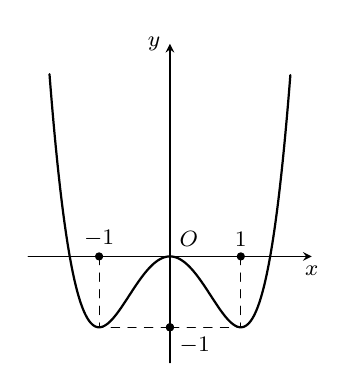
\begin{tikzpicture}[scale=0.9,>=stealth, font=\footnotesize, line join=round, line cap=round]
	%	\draw[color=gray!50,dashed] (-4,-6) grid (4,5);
	\draw[->] (-2,0)--(2,0) node [below]{$x$};
	\draw[->] (0,-1.5)--(0,3) node [left]{$y$};
	\draw[samples=300,thick,domain=-1.7:1.7]plot(\x,{(\x)^4-2*(\x)^2});
	\draw [dashed](-1,0)|-(-1,-1)|-(0,-1);
	\draw [dashed](1,0)|-(1,-1)|-(0,-1);
	\draw node at(-1,0)[above]{$-1$};
	\draw node at (1,0)[above]{$1$};
	\draw node at (0,0)[above right]{$O$};
	\draw node at (0,-1)[below right]{$-1$};
	\draw[fill=black](-1,0)circle(0.5mm);
	\draw[fill=black](1,0)circle(0.5mm);
	\draw[fill=black](0,-1)circle(0.5mm);
	\draw[fill=black](0,-1)circle(0.5mm);
	\end{tikzpicture}}}
	\loigiai{}
\end{vd}
\begin{vd}%Ví dụ 3%[Nguyễn Diệu Linh]%[2D1B3-1]
\immini{	Cho đồ thị hàm số $y=f'(x)$ như hình vẽ. 
	Hàm số $y=f(x)$ đạt giá trị nhỏ nhất trên đoạn $[0;2]$ tại $x$ bằng bao nhiêu?
	\choice
	{$x=\dfrac{2}{3}$}
	{$x=0$}
	{\True $x=1$}
	{$x=2$}}{{\color{black} \begin{tikzpicture}[scale=1.2,>=stealth, font=\footnotesize, line join=round, line cap=round]
		%	\draw[color=gray!50,dashed] (-4,-6) grid (4,5);
		\draw[->] (-2,0)--(2,0) node [below]{$x$};
		\draw[->] (0,-1.5)--(0,2) node [left]{$y$};
		\draw[samples=300,thick,domain=-1.4:1.4]plot(\x,{(\x)^3-(\x)});
		\draw node at(-1,0)[above left]{$-1$};
		\draw node at (1,0)[above]{$1$};
		\draw node at (0,0)[above right]{$O$};
		\draw[fill=black](-1,0)circle(0.5mm);
		\draw[fill=black](1,0)circle(0.5mm);
		\draw[fill=black](0,0)circle(0.5mm);
		\end{tikzpicture}}}
	\loigiai{
		Dựa vào đồ thị của hàm số $y=f'(x)$ ta có BBT như sau: 
		\begin{center}
			
\begin{tikzpicture}[scale=1]
			\tkzTabInit[nocadre=false, lgt=1.2, espcl=2.5, deltacl=0.6]{$x$/0.6, $y'$/0.6, $y$/2}{$-\infty$, $-1$, $f(0)$, $1$, $+\infty$}
			\tkzTabLine{,-,0,+,0,-,0,+,}
			\tkzTabVar{+/$$, -/$f(-1)$, +/$0$, -/$f(1)$, +/$$}
			\end{tikzpicture}
		\end{center}
		Dựa vào BBT suy ra hàm số $y=f(x)$ đạt giá trị nhỏ nhất trên đoạn $[0;2]$ tại $x=1$.}
\end{vd}
\begin{vd}%Ví dụ 4%[Nguyễn Diệu Linh]%[2D1K3-1]
\immini{	Cho hàm số $y=f(x)$ có đạo hàm là $f'(x)$. Đồ thị hàm số $y=f'(x)$ được cho như hình vẽ bên. Biết $f(0)+f(3)=f(2)+f(5)$. Giá trị nhỏ nhất và giá trị lớn nhất của $y=f(x)$ trên đoạn $[0;5]$ lần lượt là
	\choice
	{\True $f(2),f(5)$}
	{$f(0),f(5)$}
	{$f(0),f(2)$}
	{$f(1),f(5)$}}
{	{\color{black} 
		\begin{tikzpicture}[>=stealth,x=1.0cm,y=1.0cm,scale=1]
		\draw[->] (-1,0) -- (6,0) node[below] {\scriptsize $x$};
		\draw[->] (0,-1) -- (0,2) node[left] {\scriptsize $y$};
		\draw (0,0) node[below left] {\scriptsize $O$} (2,0) node[above left]{\scriptsize $2$} (5,0) node[below]{\scriptsize $5$};
		\draw[line width=0.4pt,black,dashed] (5,0)--(5,1); 
		\draw[thick,blue] plot[smooth,tension=.65] coordinates{(-0.4,1.5) (0,0) (2,0) (5,1) (5.5,1.2)};
		\end{tikzpicture}
		
}}
	\loigiai{
		Từ đồ thị $y=f'(x)$ trên đoạn $[0;5]$ ta có bảng biến thiên của hàm số $y=f(x)$: 
		\begin{center}
			
\begin{tikzpicture}[scale=1]
			\tkzTabInit[nocadre=false, lgt=1.2, espcl=2.5, deltacl=0.6]
			{$x$/0.6, $f'(x)$/0.6, $f(x)$/2}
			{$0$, $2$, $5$}
			\tkzTabLine{,-,0,+,}
			\tkzTabVar{+/$f(0)$, -/$f(2)$, +/$f(5)$}
			\end{tikzpicture}
		\end{center}
		Suy ra $\min\limits_{[0;5]} f(x)=f(2)$.\\
		Từ giả thiết, ta có: $f(0)+f(3)=f(2)+f(5)\Rightarrow f(5)-f(3)=f(0)-f(2)$.\\
		Hàm số $f(x)$ đồng biến trên $[2;5]$ \\
		$ \Rightarrow f(3)>f(2)\Rightarrow f(5)-f(2)>f(5)-f(3)=f(0)-f(2) $ nên $f(5)>f(0)$.\\
		Suy ra, $\max \limits_{[0;5]} f(x)=f(5)$.}
\end{vd}
\paragraph{Câu hỏi trắc nghiệm}
\begin{ex}%Câu 1%[Nguyễn Diệu Linh]%[2D1Y3-2]
	Giá trị lớn nhất của hàm số có bảng biến thiên sau trên tập xác định là 
	\begin{center}
		
\begin{tikzpicture}[scale=1]
		\tkzTabInit[nocadre=false, lgt=1.2, espcl=2.5, deltacl=0.6]{$x$/1, $y'$/0.6, $y$/2}{$-\infty$, $-\dfrac{1}{2}$, $2$, $+\infty$}
		\tkzTabLine{,+,0,-,0,+,}
		\tkzTabVar{-/$1$, +/$9$, -/$-1$, +/$1$}
		\end{tikzpicture}
	\end{center}
	\choice
	{$\max \limits_{\mathbb{R}} y=-1$}
	{$\max \limits_{\mathbb{R}} y=1$}
	{\True $\max \limits_{\mathbb{R}} y=9$}
	{$\max \limits_{\mathbb{R}} y=10$}
	
\end{ex}
\begin{ex}%Câu 2%[2D1Y3-2]
	Giá trị nhỏ nhất của hàm số có bảng biến thiên sau trên $[-4;+\infty)$ là 
	\begin{center}
		
\begin{tikzpicture}[scale=1]
		\tkzTabInit[nocadre=false, lgt=1.2, espcl=2.5, deltacl=0.6]{$x$/0.6, $y'$/0.6, $y$/2}{$-\infty$, $-4$, $-3$, $+\infty$}
		\tkzTabLine{,h,d,-,0,+,}
		\tkzTabVar{-H/, D+/$-8$, -/$-9$, +/$+\infty$}
		\end{tikzpicture}
	\end{center}
	\choice
	{$\min \limits_{[-4;+\infty)} y=-8$}
	{$\min \limits_{[-4;+\infty)} y=-11$}
	{$\min \limits_{[-4;+\infty)} y=-17$}
	{\True $\min \limits_{[-4;+\infty)} y=-9$}
\end{ex}
\begin{ex}%Câu 3%[Nguyễn Diệu Linh]%[2D1Y3-2]
	Giá trị lớn nhất của hàm số có bảng biến thiên sau trên khoảng $\left(\dfrac{\pi}{2};\dfrac{3\pi}{2}\right)$ là 
	\begin{center}
		
\begin{tikzpicture}[scale=1]
		\tkzTabInit[nocadre=false, lgt=1.2, espcl=2.5, deltacl=0.6]{$x$/1, $y'$/0.6, $y$/2}{$\dfrac{\pi}{2}$, $\pi$, $\dfrac{3\pi}{2}$}
		\tkzTabLine{,+,d,-,}
		\tkzTabVar{D-/$-\infty$, +/$-1$, -D/$-\infty$}
		\end{tikzpicture}
	\end{center}	
	\choice
	{Không tồn tại}
	{$1$}
	{$\pi$}
	{\True $– 1$}
\end{ex}
\begin{ex}%Câu 4%[Nguyễn Diệu Linh]%[2D1Y3-2]
	Giá trị nhỏ nhất của hàm số $y=\dfrac{1}{\sin x}$ có bảng biến thiên sau trên khoảng $(0;\pi)$ là 
	\begin{center}
		
\begin{tikzpicture}[scale=1]
		\tkzTabInit[nocadre=false, lgt=1.2, espcl=2.5, deltacl=0.6]
		{$x$/1, $y'$/0.6, $y$/2}
		{$0$, $\dfrac{\pi}{2}$, $\pi$}
		\tkzTabLine{,+,d,-,}
		\tkzTabVar{D+/$+\infty$, -/$1$, +D/$+\infty$}
		\end{tikzpicture}
	\end{center}	
	\choice
	{$-1$}
	{\True $1$}
	{$\dfrac{\pi}{2}$}
	{Không tồn tại}
\end{ex}
\begin{ex}%Câu 5%[Nguyễn Diệu Linh]%[2D1Y3-2]
	Giá trị nhỏ nhất của hàm số $y=x+\sqrt{2x^2+1}$ có bảng biến thiên sau bằng 
    \begin{center}
    	
\begin{tikzpicture}[scale=1]
    	\tkzTabInit[nocadre=false, lgt=1.2, espcl=2.5, deltacl=0.6]{$x$/1, $y'$/0.6, $y$/2}{$-\infty$, $-\dfrac{1}{\sqrt{2}}$, $+\infty$}
    	\tkzTabLine{,-,0,+,}
    	\tkzTabVar{+/$+\infty$, -/$\dfrac{1}{\sqrt{2}}$, +/$+\infty$}
    	\end{tikzpicture}
    \end{center}	
	\choice
	{\True $\min \limits_{\mathbb{R}} y=\dfrac{1}{\sqrt{2}}$}
	{$\min \limits_{\mathbb{R}} y=0$}
	{$\min \limits_{\mathbb{R}} y=1$}
	{$\min \limits_{\mathbb{R}} y=\sqrt{2}$}
\end{ex}
\begin{ex}%Câu 6%[Nguyễn Diệu Linh]%[2D1Y3-2]
	Cho hàm số $y=\sqrt{x+1}$ có bảng biến thiên sau. Khẳng định nào sau đây đúng?
	\begin{center}
		
\begin{tikzpicture}[scale=1]
		\tkzTabInit[nocadre=false, lgt=1.2, espcl=4, deltacl=0.6]{$x$/1, $y'$/0.6, $y$/1.5}{$-1$, $+\infty$}
		\tkzTabLine{d,+,}
		\tkzTabVar{-/$0$, +/$+\infty$}
		\end{tikzpicture}
	\end{center}	
	\choice
	{Hàm số không có giá trị nhỏ nhất}
	{Hàm số có giá trị lớn nhất}
	{Hàm số có giá trị nhỏ nhất bằng $-1$}
	{\True Hàm số có giá trị nhỏ nhất bằng $0$}
\end{ex}
\begin{ex}%Câu 7%[Nguyễn Diệu Linh]%[2D1Y3-1]
	Hàm số $y=\dfrac{1}{x}+ \dfrac{1}{x+1}+\dfrac{1}{x+2}$ có bảng biến thiên sau đạt giá trị lớn nhất trên đoạn $[-5;-3]$ bằng 
    \begin{center}
    	
\begin{tikzpicture}[scale=1]
    	\tkzTabInit[nocadre=false, lgt=1.2, espcl=4.5, deltacl=0.6]{$x$/1, $y'$/0.6, $y$/2.5}{$-5$, $-3$}
    	\tkzTabLine{,-,}
    	\tkzTabVar{+/$-\dfrac{47}{60}$, -/$-\dfrac{11}{6}$}
    	\end{tikzpicture}
    \end{center}	
	\choice
    {$-\dfrac{13}{12}$}
    {$\dfrac{11}{6}$}
    {\True $-\dfrac{47}{60}$}
    {$-\dfrac{11}{6}$}
\end{ex}
\begin{ex}%Câu 8%[Nguyễn Diệu Linh]%[2D1Y3-2]
	Cho hàm số $y=f(x)$ có bảng biến thiên sau. Khẳng định nào sau đây đúng?
	\begin{center}
		
\begin{tikzpicture}[scale=1]
		\tkzTabInit[nocadre=false, lgt=1.2, espcl=3, deltacl=0.6]{$x$/1, $y'$/0.6, $y$/2}{$2$, $\dfrac{5}{2}$, $+\infty$}
		\tkzTabLine{,-,0,+,}
		\tkzTabVar{+/$-6$, -/$-\dfrac{25}{4}$, +/$+\infty$}
		\end{tikzpicture}
	\end{center}	
	\choice
	{$\max\limits_{[2;+\infty]} y=-6$}
	{$\max\limits_{[2;+\infty]} y=-\dfrac{25}{4}$}
	{$\max\limits_{[2;+\infty]} y=2$}
	{\True $\min\limits_{[2;+\infty]} y=-\dfrac{25}{4}$}
\end{ex}
\begin{ex}%Câu 9%[Nguyễn Diệu Linh]%[2D1Y3-1]
\immini{	Giá trị nhỏ nhất của hàm số $y=x^3-3x+5$ có đồ thị sau trên đoạn $[0;2]$ là 
	\choice
	{$\min\limits_{[0;2]} y=0$}
	{\True $\min\limits_{[0;2]} y=1$}
	{$\min\limits_{[0;2]} y=3$}
	{$\min\limits_{[0;2]} y=5$}}{	{\color{black} 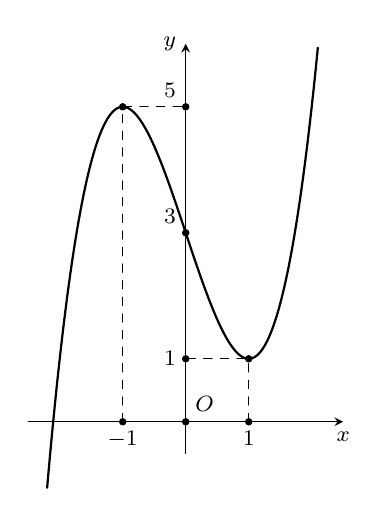
\begin{tikzpicture}[scale=0.8,>=stealth, font=\footnotesize, line join=round, line cap=round]
		%	\draw[color=gray!50,dashed] (-4,-6) grid (4,5);
		\draw[->] (-2.5,0)--(2.5,0) node [below]{$x$};
		\draw[->] (0,-0.5)--(0,6) node [left]{$y$};
		\draw[samples=300,thick,domain=-2.2:2.1]plot(\x,{(\x)^3-3*(\x)+3});
		\draw node at (0,3)[above left]{$3$};
		\draw node at (0,5)[above left]{$5$};
		\draw node at (0,1)[left]{$1$};
		\draw node at (0,0)[above right]{$O$};
		\draw node at (1,0)[below]{$1$};
		\draw node at (-1,0)[below]{$-1$};
		\draw[line width=0.4pt,black,dashed] (1,0)--(1,1)--(0,1) (-1,0)--(-1,5)--(0,5); 
		\draw[fill=black](-1,0)circle(0.5mm) (0,1)circle(0.5mm) (0,3)circle(0.5mm) (0,5)circle(0.5mm) (-1,5)circle(0.5mm) (1,1)circle(0.5mm);
		\draw[fill=black](1,0)circle(0.5mm);
		\draw[fill=black](0,0)circle(0.5mm);
		\end{tikzpicture}}}
\end{ex}
\begin{ex}%Câu 10%[Nguyễn Diệu Linh]%[2D1Y3-1]
	Giá trị lớn nhất của hàm số $f(x)=x^4-2x^2+1$ có đồ thị sau trên đoạn $[-1;1]$ là 
	\begin{center}
	{\color{black} 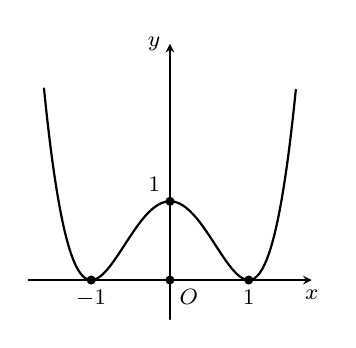
\begin{tikzpicture}[scale=1.0,>=stealth, font=\footnotesize, line join=round, line cap=round]
		%	\draw[color=gray!50,dashed] (-4,-6) grid (4,5);
		\draw[->] (-1.8,0)--(1.8,0) node [below]{$x$};
		\draw[->] (0,-0.5)--(0,3) node [left]{$y$};
		\draw[samples=300,thick,domain=-1.6:1.6]plot(\x,{(\x)^4-2*(\x)^2+1});
		\draw node at (0,1)[above left]{$1$};
		\draw node at (0,0)[below right]{$O$};
		\draw node at (1,0)[below]{$1$};
		\draw node at (-1,0)[below]{$-1$};
		\draw[fill=black](-1,0)circle(0.5mm) (0,1)circle(0.5mm) (1,0)circle(0.5mm) (0,0)circle(0.5mm);
		\end{tikzpicture}}
\end{center}
	\choice
	{$\max\limits_{[-1; 1]} f(x)=0$}
	{$\max\limits_{[-1; 1]} f(x)=2$}
	{$\max\limits_{[-1; 1]} f(x)=-1$}
	{\True $\max\limits_{[-1; 1]} f(x)=1$}
\end{ex}
\begin{ex}%Câu 11%[Nguyễn Diệu Linh]%[2D1B3-2]
	Cho hàm số $y=x-\sqrt{x-1}$ có bảng biến thiên sau. Khẳng định nào sau đây đúng?
	\begin{center}
		
\begin{tikzpicture}[scale=1]
		\tkzTabInit[nocadre=false, lgt=1.2, espcl=3, deltacl=0.6]{$x$/1, $y'$/0.6, $y$/2}{$1$, $\dfrac{5}{4}$, $+\infty$}
		\tkzTabLine{,-,0,+,}
		\tkzTabVar{+/$1$, -/$\dfrac{3}{4}$, +/$0$}
		\end{tikzpicture}
	\end{center}	
	\choice
	{Hàm số có giá trị nhỏ nhất bằng $\dfrac{3}{4}$ và không có giá trị lớn nhất}
	{\True Hàm số có giá trị nhỏ nhất bằng $\dfrac{3}{4}$ và giá trị lớn nhất bằng $1$}
	{Hàm số không có giá trị lớn nhất và giá trị nhỏ nhất}
	{Hàm số đạt giá trị nhỏ nhất tại điểm có hoành độ $x=1$ và giá trị nhỏ nhất bằng $1$}
\end{ex}
\begin{ex}%Câu 12%[Nguyễn Diệu Linh]%[2D1B3-1]
	Cho hàm số $y=\dfrac{x-1}{x+1}$ có đồ thị sau. Chọn khẳng định đúng?
	\begin{center}
		{\color{black} % Đồ thị hàm y=(ax+b)/(cx+d), ad-bc khác 0. Nếu hệ số lớn cần điều chỉnh hệ trục, vùng lưới, domain và lệnh \clip
			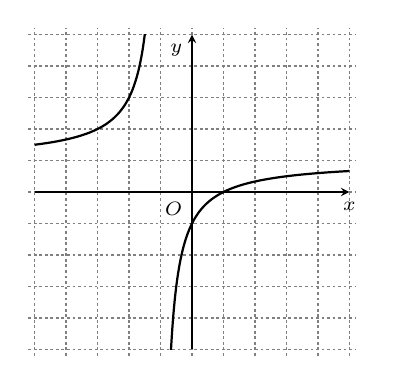
\begin{tikzpicture}[>=stealth,x=1cm,y=1cm,scale=0.4]
			\def\a{1}
			\def\b{-1}
			\def\c{1}
			\def\d{1}
			\draw[color=gray,dash pattern=on 1pt off 1pt,xstep=1.0cm,ystep=1.0cm] (-5.2,-5.2) grid (5.2,5.2);
			\draw[->] (-5,0) -- (5,0) node[below] {\scriptsize $x$};
			\draw[->] (0,-5) -- (0,5) node[below left] {\scriptsize $y$};
			\draw (0,0)node[below left]{\scriptsize $O$};
			\clip (-5,-5)rectangle(5,5);
			\pgfmathsetmacro{\can}{-(\d)/(\c)}
			\draw[thick,samples=150,smooth,domain=-5:{\can-.1}] plot(\x,{(\a*\x+(\b))/(\c*\x+(\d))}); % Vẽ nhánh bên trái TCĐ
			\draw[thick,samples=150,smooth,domain={\can+.1}:5] plot(\x,{(\a*\x+(\b))/(\c*\x+(\d))}); % Vẽ nhánh bên phải TCĐ
			\fill[black] (0,-1) circle (1.5pt) (1,0) circle (1.5pt);
			\end{tikzpicture}
		}
	\end{center}
	\choice
	{$\max\limits_{[0; 3]} y=-3$}
	{$\min\limits_{[-1; 3]} y=3$}
	{\True $\min\limits_{[0; 3]} y=-1$}
	{$\max\limits_{[0; 4]} y=-3$}
\end{ex}
\begin{ex}%Câu 13%[Nguyễn Diệu Linh]%[2D1B3-1]
	Cho hàm số $y=x+\dfrac{1}{x}$ có đồ thị sau. Chọn phát biểu đúng?
	\begin{center}
		{\color{black} 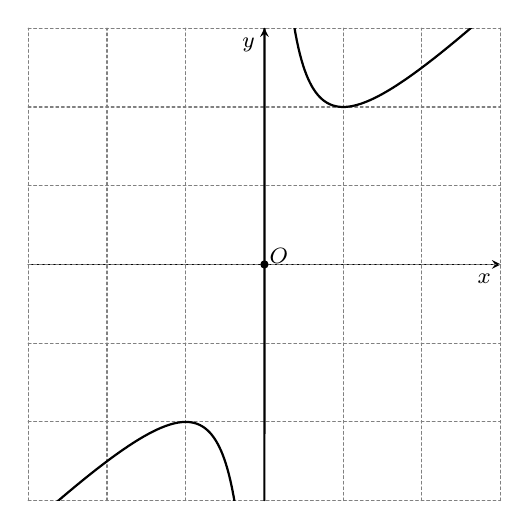
\begin{tikzpicture}[scale=1.0,>=stealth, font=\footnotesize, line join=round, line cap=round]
			\draw[->] (-3,0)--(3,0) node [below left]{$x$};
			\draw[->] (0,-3)--(0,3) node [below left]{$y$};
			\draw[color=gray,dash pattern=on 1pt off 1pt,xstep=1.0cm,ystep=1.0cm] (-3,-3) grid (3,3);
			\clip (-3,-3)rectangle(3,3);
			\draw[samples=300,thick,domain=-3:3]plot(\x,{(\x)+1/(\x)});
			\fill[black] (0,0)node[shift={(30:6pt)}]{$O$} circle (1.5pt); % Nhãn điểm ở hướng 30 độ, bán kính 6pt của điểm A
			
			\end{tikzpicture}}
	\end{center}
	\choice
	{\True $\min\limits_{[0;2]} y+\max\limits_{[-2;0]} y=0$}
	{$\min\limits_{[0;2]} y+\max\limits_{[-2;0]} y=4$}
	{$\min\limits_{[0;2]} y+\max\limits_{[-2;0]} y=-4$}
	{$\min\limits_{[0;2]} y+\max\limits_{[-2;0]} y=2$}
	\loigiai{
Dựa vào đồ thị, ta thấy $\min\limits_{[0;2]}=2$, $\max\limits_{[-2;0]} y=-2$ nên $\min\limits_{[0;2]} y+\max\limits_{[-2;0]} y=0$.
}
\end{ex}
\begin{ex}%Câu 14%[Nguyễn Diệu Linh]%[2D1B3-1]
	Gọi $y_1;y_2$ lần lượt là giá trị lớn nhất, giá trị nhỏ nhất của hàm số $y=\dfrac{1}{x-1}+\dfrac{1}{x-2}$ có bảng biến thiên sau trên đoạn $[3;4]$. Khi đó tích $y_1\cdot y_2$ là bao nhiêu?
     \begin{center}
    	
\begin{tikzpicture}[scale=1]
    	\tkzTabInit[nocadre=false, lgt=1.2, espcl=4.5, deltacl=0.6]
    	{$x$/0.7, $y'$/0.7, $y$/2.1}
    	{$3$, $4$}
    	\tkzTabLine{,-,}
    	\tkzTabVar{+/$\dfrac{3}{2}$, -/$\dfrac{5}{6}$}
    	\end{tikzpicture}
    \end{center}	
	\choice
	{$\dfrac{3}{2}$}
	{$\dfrac{5}{6}$}
	{\True $\dfrac{5}{4}$}
	{$\dfrac{7}{3}$}
	\loigiai{
	Dựa vào bảng biến thiên, ta thấy $y_1=\dfrac{3}{2}$, $y_2=\dfrac{5}{6}$.}
\end{ex}
\begin{ex}%Câu 15%[Nguyễn Diệu Linh]%[2D1B3-1]
	Cho hàm số $y=f(x)$ có bảng biến thiên sau. Hàm số đạt giá trị lớn nhất là $f(x_0)$ tại $x_0$. Khi đó tích $x_0\cdot f(x_0)$ bằng 
	\begin{center}
		
\begin{tikzpicture}[scale=1]
		\tkzTabInit[nocadre=false, lgt=1.2, espcl=2.5, deltacl=0.6]{$x$/0.6, $f'(x)$/0.6, $f(x)$/2}{$0$, $4$, $8$}
		\tkzTabLine{,+,0,-,}
		\tkzTabVar{-/$0$, +/$16$, -/$0$}
		\end{tikzpicture}
	\end{center}	
	\choice
	{\True $64$}
	{$4$}
	{$0$}
	{$20$}
	\loigiai{
Dựa vào bảng biến thiên, ta thấy, hàm số đạt giá trị lớn nhất là $16$ tại $x=4$ nên $x_0\cdot f(x_0)=64$.
}
\end{ex}
\begin{ex}%Câu 16%[Nguyễn Diệu Linh]%[2D1B3-1]
	Cho hàm số $y=f(x)$ có bảng biến thiên sau. Hàm số đạt giá trị nhỏ nhất là $f(x_0)$ tại $x_0$. Khi đó $x_0+f(x_0)$ bằng 
	\begin{center}
		
\begin{tikzpicture}[scale=1]
		\tkzTabInit[nocadre=false, lgt=1.2, espcl=2.5, deltacl=0.6]{$x$/0.6, $f'(x)$/0.6, $f(x)$/2}{$0$, $4\sqrt{3}$, $48$}
		\tkzTabLine{,-,0,+,}
		\tkzTabVar{+/$f(0)$, -/$16\sqrt{3}$, +/$f(48)$}
		\end{tikzpicture}
	\end{center}	
	\choice
	{$16\sqrt{3}$}
	{\True $20\sqrt{3}$}
	{$20$}
	{$8\sqrt{3}$}
	\loigiai{
Dựa vào bảng biến thiên ta thấy, hàm số đạt giá trị nhỏ nhất là $16\sqrt{3}$ tại $4\sqrt{3}$ nên $x_0+f(x_0)=20\sqrt{3}$.	
}
\end{ex}
\begin{ex}%Câu 17%[Nguyễn Diệu Linh]%[2D1B3-1]
	Cho hàm số $y=f(x)$ có bảng biến thiên sau. Hàm số đạt giá trị nhỏ nhất là $f(x_0)$ tại $x_0$. Khi đó $x_0^2+f(x_0)$ bằng 
	\begin{center}
		
\begin{tikzpicture}[scale=1]
		\tkzTabInit[nocadre=false, lgt=1.2, espcl=3, deltacl=0.6]
		{$x$/1, $f'(x)$/0.6, $f(x)$/2.5}
		{$-\infty$, $-\dfrac{13}{2}$, $+\infty$}
		\tkzTabLine{,-,0,+,}
		\tkzTabVar{+/$+\infty$,  -/$-\dfrac{169}{4}$, +/$+\infty$}
		\end{tikzpicture}
	\end{center}	
	\choice
	{$-\dfrac{169}{2}$}
	{$-\dfrac{169}{4}$}
	{\True $0$}
	{$\dfrac{169}{2}$}
	\loigiai{
		Dựa vào bảng biến thiên ta thấy, hàm số đạt giá trị nhỏ nhất là $-\dfrac{169}{4}$ tại $-\dfrac{13}{2}$ nên $x_0^2+f(x_0)=0$.	
	}
\end{ex}
\begin{ex}%Câu 18%[Nguyễn Diệu Linh]%[2D1B3-1]
	Cho hàm số $y=f(x)$ có bảng biến thiên sau. Tìm $a$ để hàm số có giá trị lớn nhất trên đoạn $[0;10]$ là $2\sqrt{3}$. 
	\begin{center}
		
\begin{tikzpicture}[scale=1]
		\tkzTabInit[nocadre=false, lgt=1.2, espcl=3, deltacl=0.6]{$x$/1, $f'(x)$/0.6, $f(x)$/2.5}{$0$, $\dfrac{a}{3}$, $10$}
		\tkzTabLine{,+,0,-,}
		\tkzTabVar{-/$f(0)$, +/$\dfrac{a^2}{6\sqrt{3}}$, -/$f(10)$}
		\end{tikzpicture}
	\end{center}	
	\choice
	{$6\sqrt{3}$}
	{$36$}
	{$36\sqrt{3}$}
	{\True $6$}
	\loigiai{
Dựa vào bảng biến thiên, ta thấy, hàm số đạt giá trị lớn nhất trên đoạn $[0;10]$ là $\dfrac{a^2}{6\sqrt{3}}$.\\
$\dfrac{a^2}{6\sqrt{3}}=2\sqrt{3}\Leftrightarrow a^2=36 \Leftrightarrow \hoac{a=6\\}a=-6.$	
}
\end{ex}
\begin{ex}%Câu 19%[Nguyễn Diệu Linh]%[2D1B3-1]
	Cho hàm số $y=f(x)$ có bảng biến thiên sau. Tìm $a$ để hàm số có giá trị lớn nhất trên đoạn $[0;20]$ là $8$. 
    \begin{center}
    	
\begin{tikzpicture}[scale=1]
    	\tkzTabInit[nocadre=false, lgt=1.2, espcl=3, deltacl=0.6]{$x$/1, $f'(x)$/0.6, $f(x)$/2.5}{$0$, $\dfrac{a}{4}$, $20$}
    	\tkzTabLine{,+,0,-,}
    	\tkzTabVar{-/$f(0)$, +/$\dfrac{a^2}{8}$, -/$f(20)$}
    	\end{tikzpicture}
    \end{center}	
	\choice
	{$4$}
	{$16$}
	{\True $8$}
	{$4\sqrt{2}$}
	\loigiai{
		Dựa vào bảng biến thiên, ta thấy, hàm số đạt giá trị lớn nhất trên đoạn $[0;20]$ là $\dfrac{a^2}{8}$.\\
		$\dfrac{a^2}{8}=8\Leftrightarrow a^2=64 \Leftrightarrow \hoac{a=8\\a=-8.}$	
	}
\end{ex}
\begin{ex}%Câu 20%[Nguyễn Diệu Linh]%[2D1B3-1]
\immini{	Hàm số $y=x^3-3x+1$ có đồ thị như hình vẽ đạt giá trị lớn nhất và giá trị nhỏ nhất trên đoạn $\left[-\dfrac{3}{2};\dfrac{3}{2}\right]$ tại điểm có hoành độ lần lượt là $x_1;x_2$. Khi đó tổng $x_1+x_2$ bằng 
	\choice
	{$2$}
	{$1$}
	{$3$}
	{\True $0$}}
{	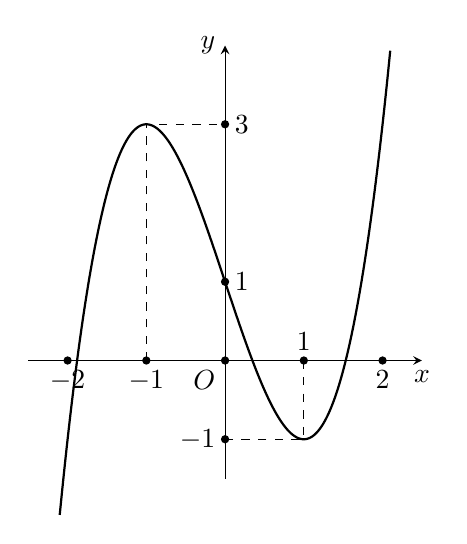
\begin{tikzpicture}[>=stealth,x=1cm,y=1cm,scale=1]
	\draw[->] (-2.5,0)--(2.5,0) node [below]{$x$};
	\draw[->] (0,-1.5)--(0,4) node [left]{$y$};
	\draw[samples=300,thick,domain=-2.1:2.1]plot(\x,{(\x)^3-3*(\x)+1});
	\draw[dashed](1,0)--(1,-1)--(0,-1) (-1,0)--(-1,3)--(0,3);
	\fill[black] (2,0)node[below]{$2$} circle (1.5pt) (1,0)node[above]{$1$} circle (1.5pt) (-1,0)node[below]{$-1$} circle (1.5pt) (-2,0)node[below]{$-2$} circle (1.5pt) (0,0)node[below left]{$O$} circle (1.5pt) (0,1)node[right]{$1$} circle (1.5pt) (0,3)node[right]{$3$} circle (1.5pt) (0,-1)node[left]{$-1$} circle (1.5pt);
	\end{tikzpicture}}
\loigiai{
Dựa vào đồ thị, ta thấy $x_1=-1$, $x_2=1$ tổng $x_1+x_2=0$.
}
\end{ex}
\begin{ex}%Câu 21%[Nguyễn Diệu Linh]%[2D1K3-1]
\immini{	Cho đồ thị hàm số $y=f'(x)$ như hình vẽ. 
	Hàm số $y=f(x)$ đạt giá trị lớn nhất trên đoạn $[-1;1]$ tại $x$ bằng bao nhiêu?
	\choice
	{$x=\dfrac{2}{3}$}
	{\True $x=0$}
	{$x=1$}
	{$x=2$}}{
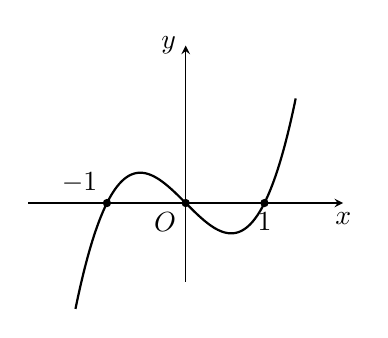
\begin{tikzpicture}[>=stealth,x=1cm,y=1cm,scale=1]
\draw[->] (-2,0)--(2,0) node [below]{$x$};
\draw[->] (0,-1)--(0,2) node [left]{$y$};
\draw[samples=300,thick,domain=-1.4:1.4]plot(\x,{(\x)^3-(\x)});
\fill[black] (1,0)node[below]{$1$} circle (1.5pt) (-1,0)node[above left]{$-1$} circle  (1.5pt) (0,0)node[below left]{$O$} circle (1.5pt);
\end{tikzpicture}}
	\loigiai{
		Dựa vào đồ thị của hàm số $y=f'(x)$ ta có BBT như sau: 
	    \begin{center}
	    	
\begin{tikzpicture}[scale=1]
	    	\tkzTabInit[nocadre=false, lgt=1.2, espcl=2.5, deltacl=0.6]{$x$/0.6, $f'(x)$/0.6, $f(x)$/2}{$-\infty$, $-1$, $0$, $1$, $+\infty$}
	    	\tkzTabLine{,-,0,+,0,-,0,+,}
	    	\tkzTabVar{+/$+\infty$, -/$f(-1)$, +/$0$, -/$f(1)$, +/$+\infty$}
	    	\end{tikzpicture}
	    \end{center}	
		Dựa vào BBT suy ra hàm số $y=f(x)$ đạt giá trị lớn nhất trên đoạn $[-1;1]$ tại $x=0$.}
\end{ex}
\begin{ex}%Câu 22%[Nguyễn Diệu Linh]%[2D1K3-1]
\immini{	Cho đồ thị hàm số $y=f'(x)$ như hình vẽ. 
	Hàm số $y=f(x)$ đạt giá trị nhỏ nhất trên đoạn $[-1;4]$ tại $x$ bằng bao nhiêu?
	\choice
	{\True $x=3$}
	{$x=0$}
	{$x=4$}
	{$x=-1$}}
{{\color{black} 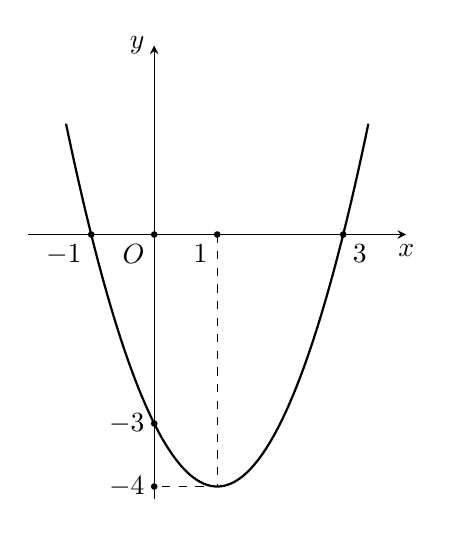
\begin{tikzpicture}[>=stealth,x=1cm,y=1cm,scale=0.8]
		\draw[->] (-2,0)--(4,0) node [below]{$x$};
		\draw[->] (0,-4.2)--(0,3) node [left]{$y$};
		\draw[samples=300,thick,domain=-1.4:3.4]plot(\x,{(\x)^2-2*(\x)-3});
		\fill[black] (3,0)node[below right]{$3$} circle (1.5pt) (-1,0)node[below left]{$-1$} circle  (1.5pt) (0,0)node[below left]{$O$} circle (1.5pt) (0,-3)node[left]{$-3$} circle (1.5pt) (0,-4)node[left]{$-4$} circle (1.5pt) (1,0)node[below left]{$1$} circle  (1.5pt);
		\draw[line width=0.4pt,black,dashed] (1,0)--(1,-4)--(0,-4);
		\end{tikzpicture}}}
	\loigiai{
		Dựa vào đồ thị của hàm số $y=f'(x)$ ta có BBT như sau: 
	    \begin{center}
	    	
\begin{tikzpicture}[scale=1]
	    	\tkzTabInit[nocadre=false, lgt=1.5, espcl=2.0, deltacl=0.8]{$x$/0.6, $y'$/0.6, $y$/2}{$-1$, $3$, $4$}
	    	\tkzTabLine{0,-,0,+,}
	    	\tkzTabVar{+/$f(-1)$, -/$f(3)$, +/$f(4)$}
	    	\end{tikzpicture}
	    \end{center}	
		Dựa vào BBT suy ra hàm số $y=f(x)$ đạt giá trị nhỏ nhất trên đoạn $[-1;4]$ tại $x=3$.}
\end{ex}
\begin{ex}%Câu 23%[Nguyễn Diệu Linh]%[2D1K3-1]
\immini{	Cho đồ thị hàm số $y=f'(x)$ như hình vẽ. 
	Hàm số $y=f(x)$ đạt giá trị nhỏ nhất trên đoạn $[0;3]$ tại $x$ bằng bao nhiêu?
	\choice
	{$x=3$}
	{$x=0$}
	{$x=2$}
	{\True $x=1$}}{{\color{black} 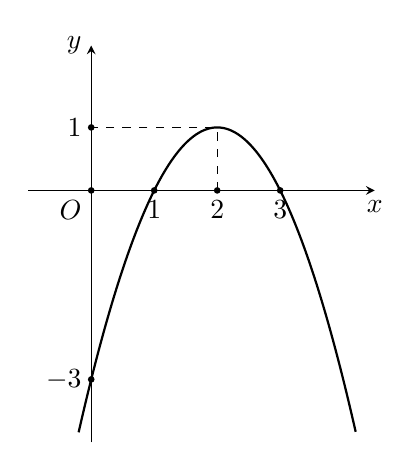
\begin{tikzpicture}[>=stealth,x=1cm,y=1cm,scale=0.8]
		\draw[->] (-1,0)--(4.5,0) node [below]{$x$};
		\draw[->] (0,-4)--(0,2.3) node [left]{$y$};
		\draw[samples=300,thick,domain=-0.2:4.2]plot(\x,{-(\x)^2+4*(\x)-3});
		\fill[black] (3,0)node[below]{$3$} circle (1.5pt) (0,-3)node[left]{$-3$} circle (1.5pt) (1,0)node[below]{$1$} circle  (1.5pt) (0,1)node[left]{$1$} circle (1.5pt) (2,0)node[below]{$2$} circle (1.5pt) (0,0)node[below left]{$O$} circle (1.5pt);
		\draw[line width=0.4pt,black,dashed] (2,0)--(2,1)--(0,1); 
		\end{tikzpicture}}}
	\loigiai{
		Dựa vào đồ thị của hàm số $y=f'(x)$ ta có BBT như sau: 
		\begin{center}
			
\begin{tikzpicture}[scale=1]
			\tkzTabInit[nocadre=false, lgt=1.2, espcl=2.5, deltacl=0.6]{$x$/0.6, $y'$/0.6, $y$/2}{$0$, $1$, $3$}
			\tkzTabLine{,-,0,+,0}
			\tkzTabVar{+/$f(0)$, -/$f(1)$, +/$f(3)$}
			\end{tikzpicture}
		\end{center}	
		Dựa vào BBT suy ra hàm số $y=f(x)$ đạt giá trị nhỏ nhất trên đoạn $[0;3]$ tại $x=1$.}
\end{ex}
\begin{ex}%Câu 24%[Nguyễn Diệu Linh]%[2D1K3-1]
	Cho đồ thị hàm số $y=f'(x)$ như hình vẽ.
	\begin{center}
	{\color{black} 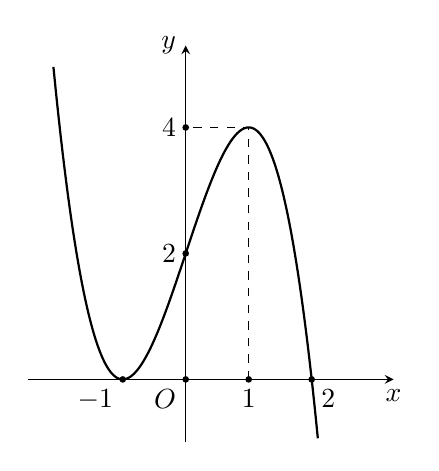
\begin{tikzpicture}[>=stealth,x=1cm,y=1cm,scale=0.8]
		\draw[->] (-2.5,0)--(3.3,0) node [below]{$x$};
		\draw[->] (0,-1)--(0,5.3) node [left]{$y$};
		\draw[samples=300,thick,domain=-2.1:2.1]plot(\x,{-(\x)^3+3*(\x)+2});
		\fill[black] (2,0)node[below right]{$2$} circle (1.5pt) (0,4)node[left]{$4$} circle (1.5pt) (1,0)node[below]{$1$} circle  (1.5pt)
		(-1,0)node[below left]{$-1$} circle  (1.5pt) (0,2)node[left]{$2$} circle (1.5pt) (0,0)node[below left]{$O$} circle (1.5pt);
		\draw[line width=0.4pt,black,dashed] (1,0)--(1,4)--(0,4); 
		\end{tikzpicture}}
	\end{center} 
	Hàm số $y=f(x)$ đạt giá trị lớn nhất trên đoạn $[-2;2]$ tại $x$ bằng bao nhiêu?
	\choice
	{\True $x=2$}
	{$x=0$}
	{$x=-2$}
	{$x=1$}
	\loigiai{
		Dựa vào đồ thị của hàm số $y=f'(x)$ ta có BBT như sau: 
		\begin{center}
			
\begin{tikzpicture}[scale=1]
			\tkzTabInit[nocadre=false, lgt=1.2, espcl=2.5, deltacl=0.8]{$x$/0.6, $y'$/0.6, $y$/2}{$-2$, $-1$, $2$}
			\tkzTabLine{,+,0,+,0}
			\tkzTabVar{-/$f(-2)$,R, +/$f(2)$}
			\end{tikzpicture}
		\end{center}	
		Dựa vào BBT suy ra hàm số $y=f(x)$ đạt giá trị lớn nhất trên đoạn $[-2;2]$ tại $x=2$.}
\end{ex}
\begin{ex}%Câu 25%[Nguyễn Diệu Linh]%[2D1K3-1]
	Cho đồ thị hàm số $y=f'(x)$ như hình vẽ. 
\begin{center}
	{\color{black} %
		% Đồ thị đi qua các điểm cụ thể
		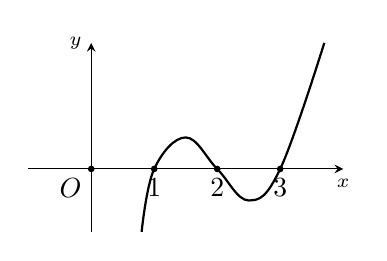
\begin{tikzpicture}[>=stealth,x=1.0cm,y=1.0cm,scale=0.8]
		\draw[->] (-1,0) -- (4,0) node[below] {\scriptsize $x$};
		\draw[->] (0,-1) -- (0,2) node[left] {\scriptsize $y$};
		\draw[thick,black] plot[smooth,tension=.65] coordinates{(0.8,-1) (1,-0) (1.5,0.5) (2,0) (2.5,-0.5) (3,0) (3.7,2)};
		\fill[black] (1,0)node[below]{$1$} circle (1.5pt) (2,0)node[below]{$2$} circle (1.5pt) (3,0)node[below]{$3$} circle (1.5pt) (0,0)node[below left]{$O$} circle (1.5pt); % Nhãn điểm ở hướng 30 độ, bán kính 6pt của điểm A
		
		\end{tikzpicture}
	}
\end{center} 
	Hàm số $y=f(x)$ đạt giá trị lớn nhất trên đoạn $[1;3]$ tại $x_0$. Khi đó giá trị của $x_0^2-2x_0+2018$ bằng bao nhiêu?
	\choice
	{\True $2018$}
	{$2017$}
	{$2021$}
	{$2026$}
	\loigiai{
		Dựa vào đồ thị của hàm số $y=f'(x)$ ta có BBT như sau: 
		\begin{center}
			
\begin{tikzpicture}[scale=1]
			\tkzTabInit[nocadre=false, lgt=1.2, espcl=2.5, deltacl=0.6]{$x$/0.6, $y'$/0.6, $y$/2}{$1$, $2$, $3$}
			\tkzTabLine{0,+,0,-,0}
			\tkzTabVar{-/$f(1)$, +/$f(2)$, -/$f(3)$}
			\end{tikzpicture}
		\end{center}	
		Dựa vào BBT suy ra hàm số $y=f(x)$ đạt giá trị lớn nhất trên đoạn $[1;3]$ tại $x_0=2$.\\
		Nên $x_0^2-2x_0+2018=2018$.}
\end{ex}
\Closesolutionfile{ans}